\documentclass{article}

\usepackage[utf8]{inputenc}
\usepackage[T1]{fontenc}
\usepackage[francais]{babel}
\usepackage{titling}
\setlength{\droptitle}{-3cm}
\usepackage{graphicx}
\usepackage{underscore}
\usepackage{hyperref} 


\title{Compte rendu : Jour 3}
\author{CAROT Axel, ARISOY Ivan Can, \\ BREILLAD Matis, BELKHITER Medhi}
\date{\today}

\begin{document}
\maketitle

\section{Travail effectué}

\subsection{Site}

\begin{figure}[h]
    \centering
    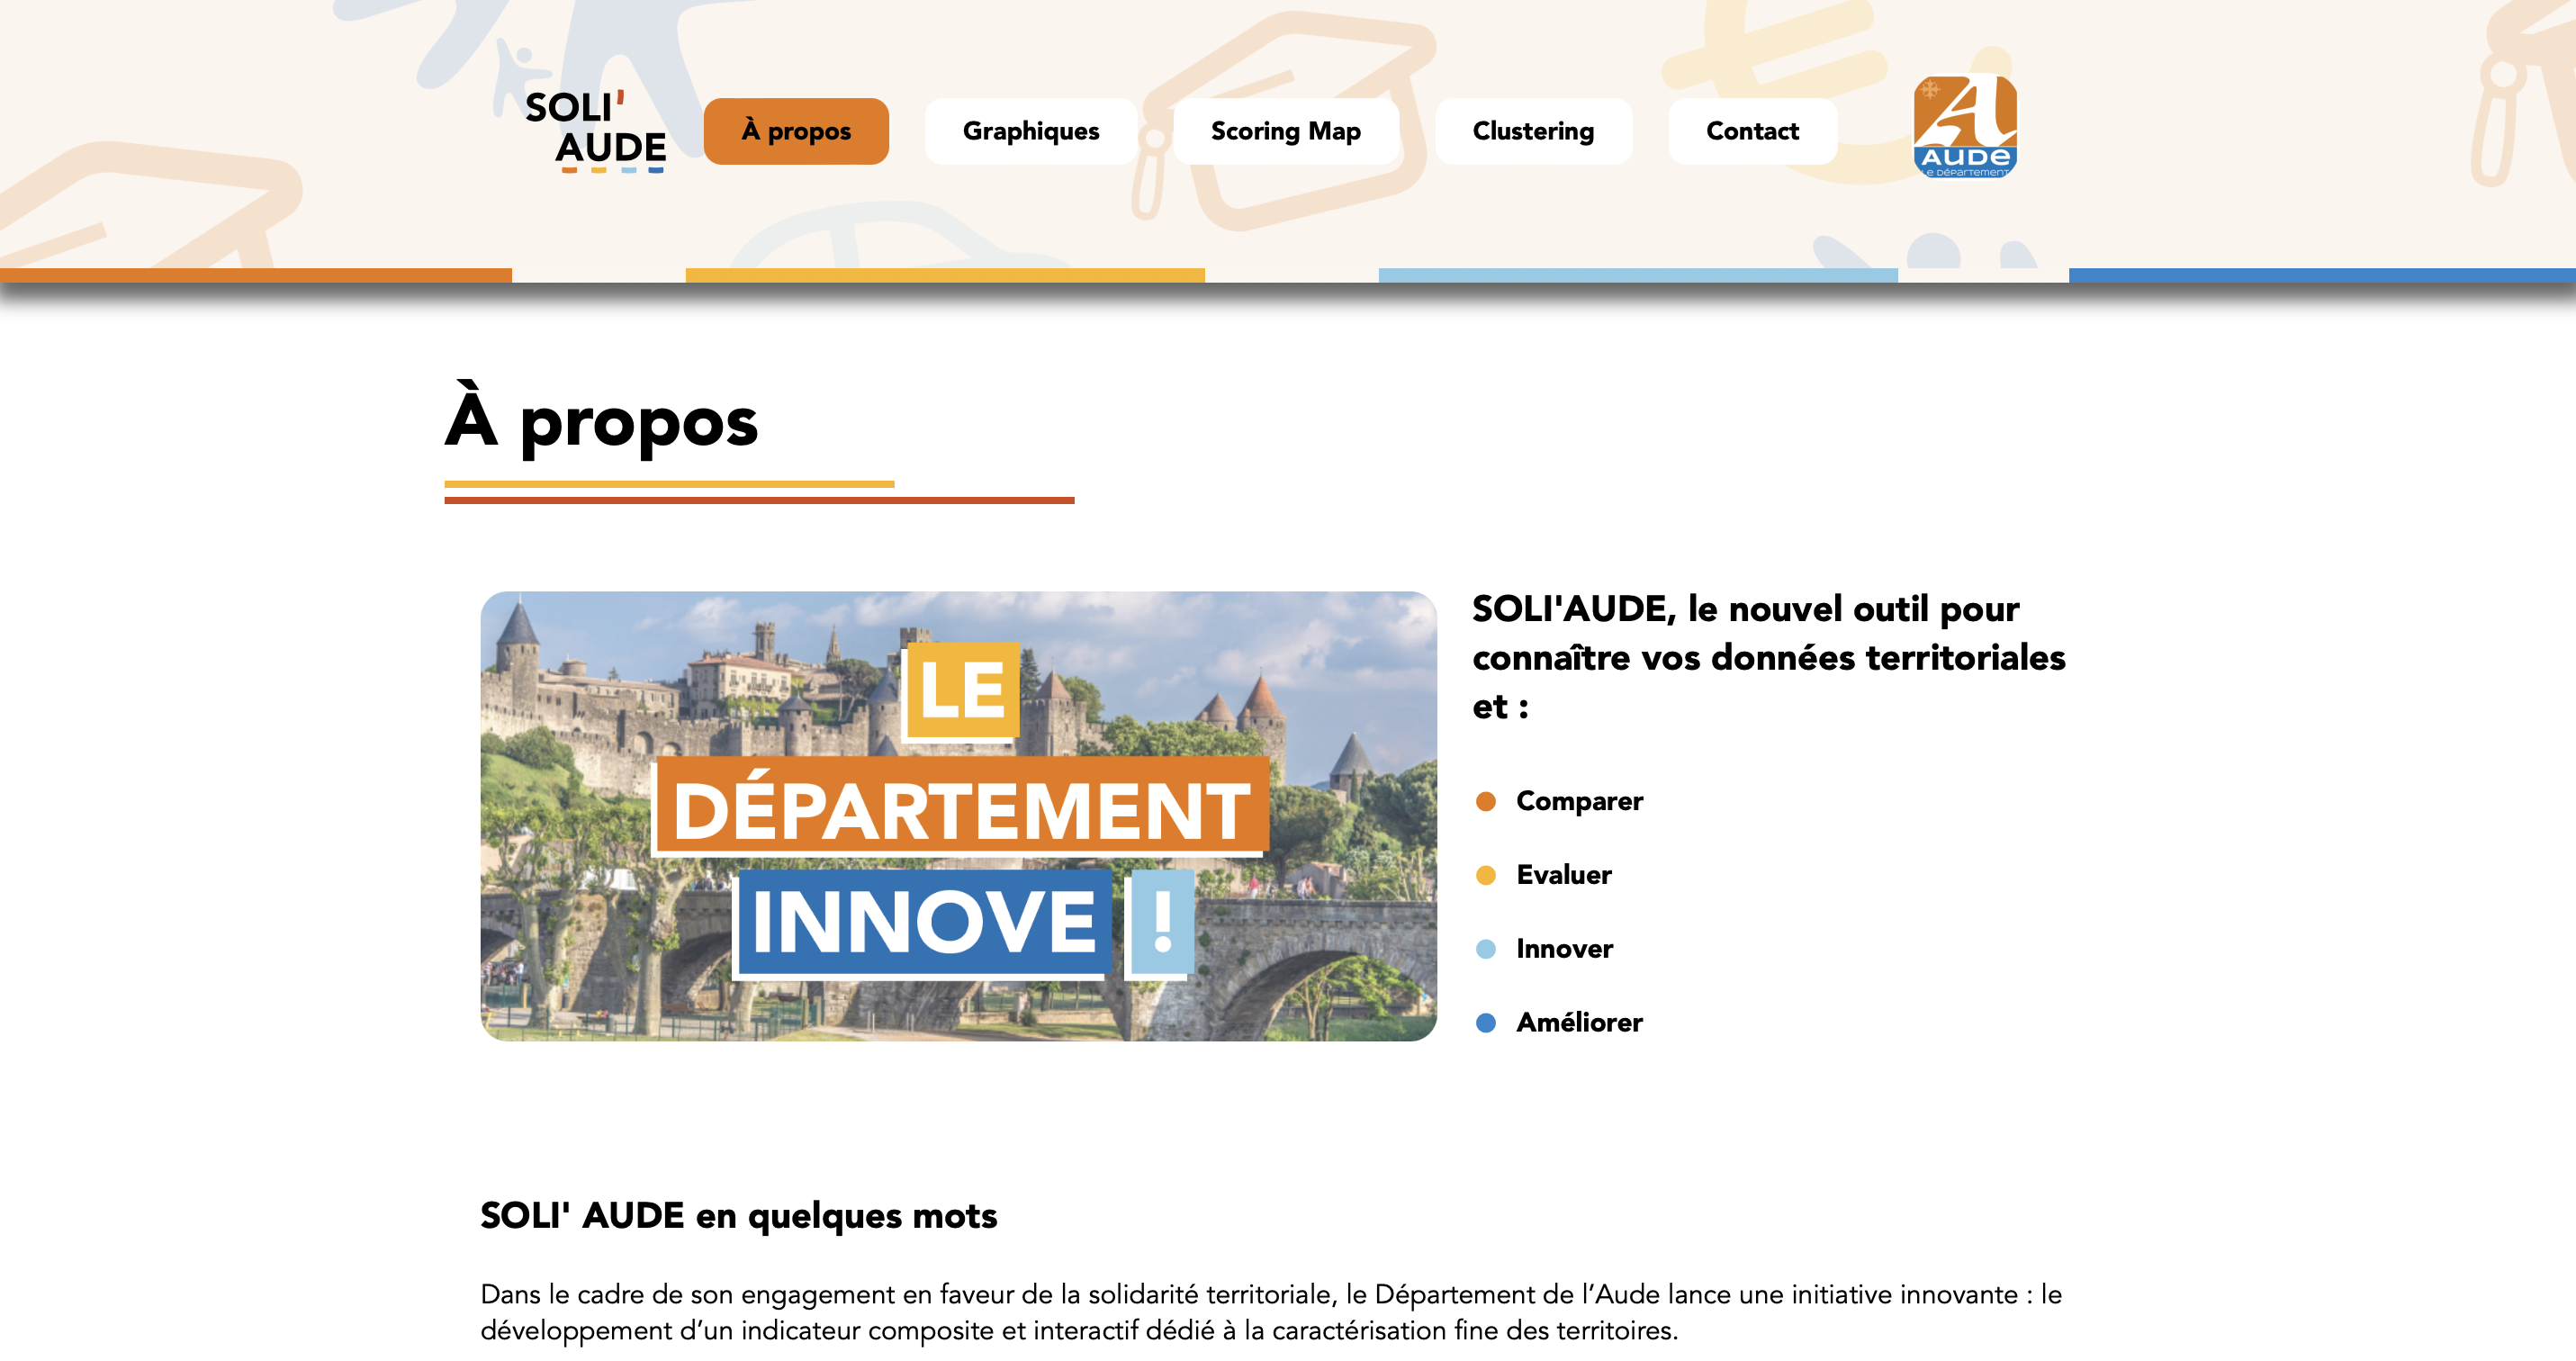
\includegraphics[width=0.6\textwidth]{1.png}
    \caption{Page d'acceuil}
    \label{fig:Page d'acceuil}
\end{figure}

Nous avons étoffé le design/front-end du site pour s'accorder avec la charte graphique de l'équipe des CNO.

\begin{figure}[h]
    \centering
    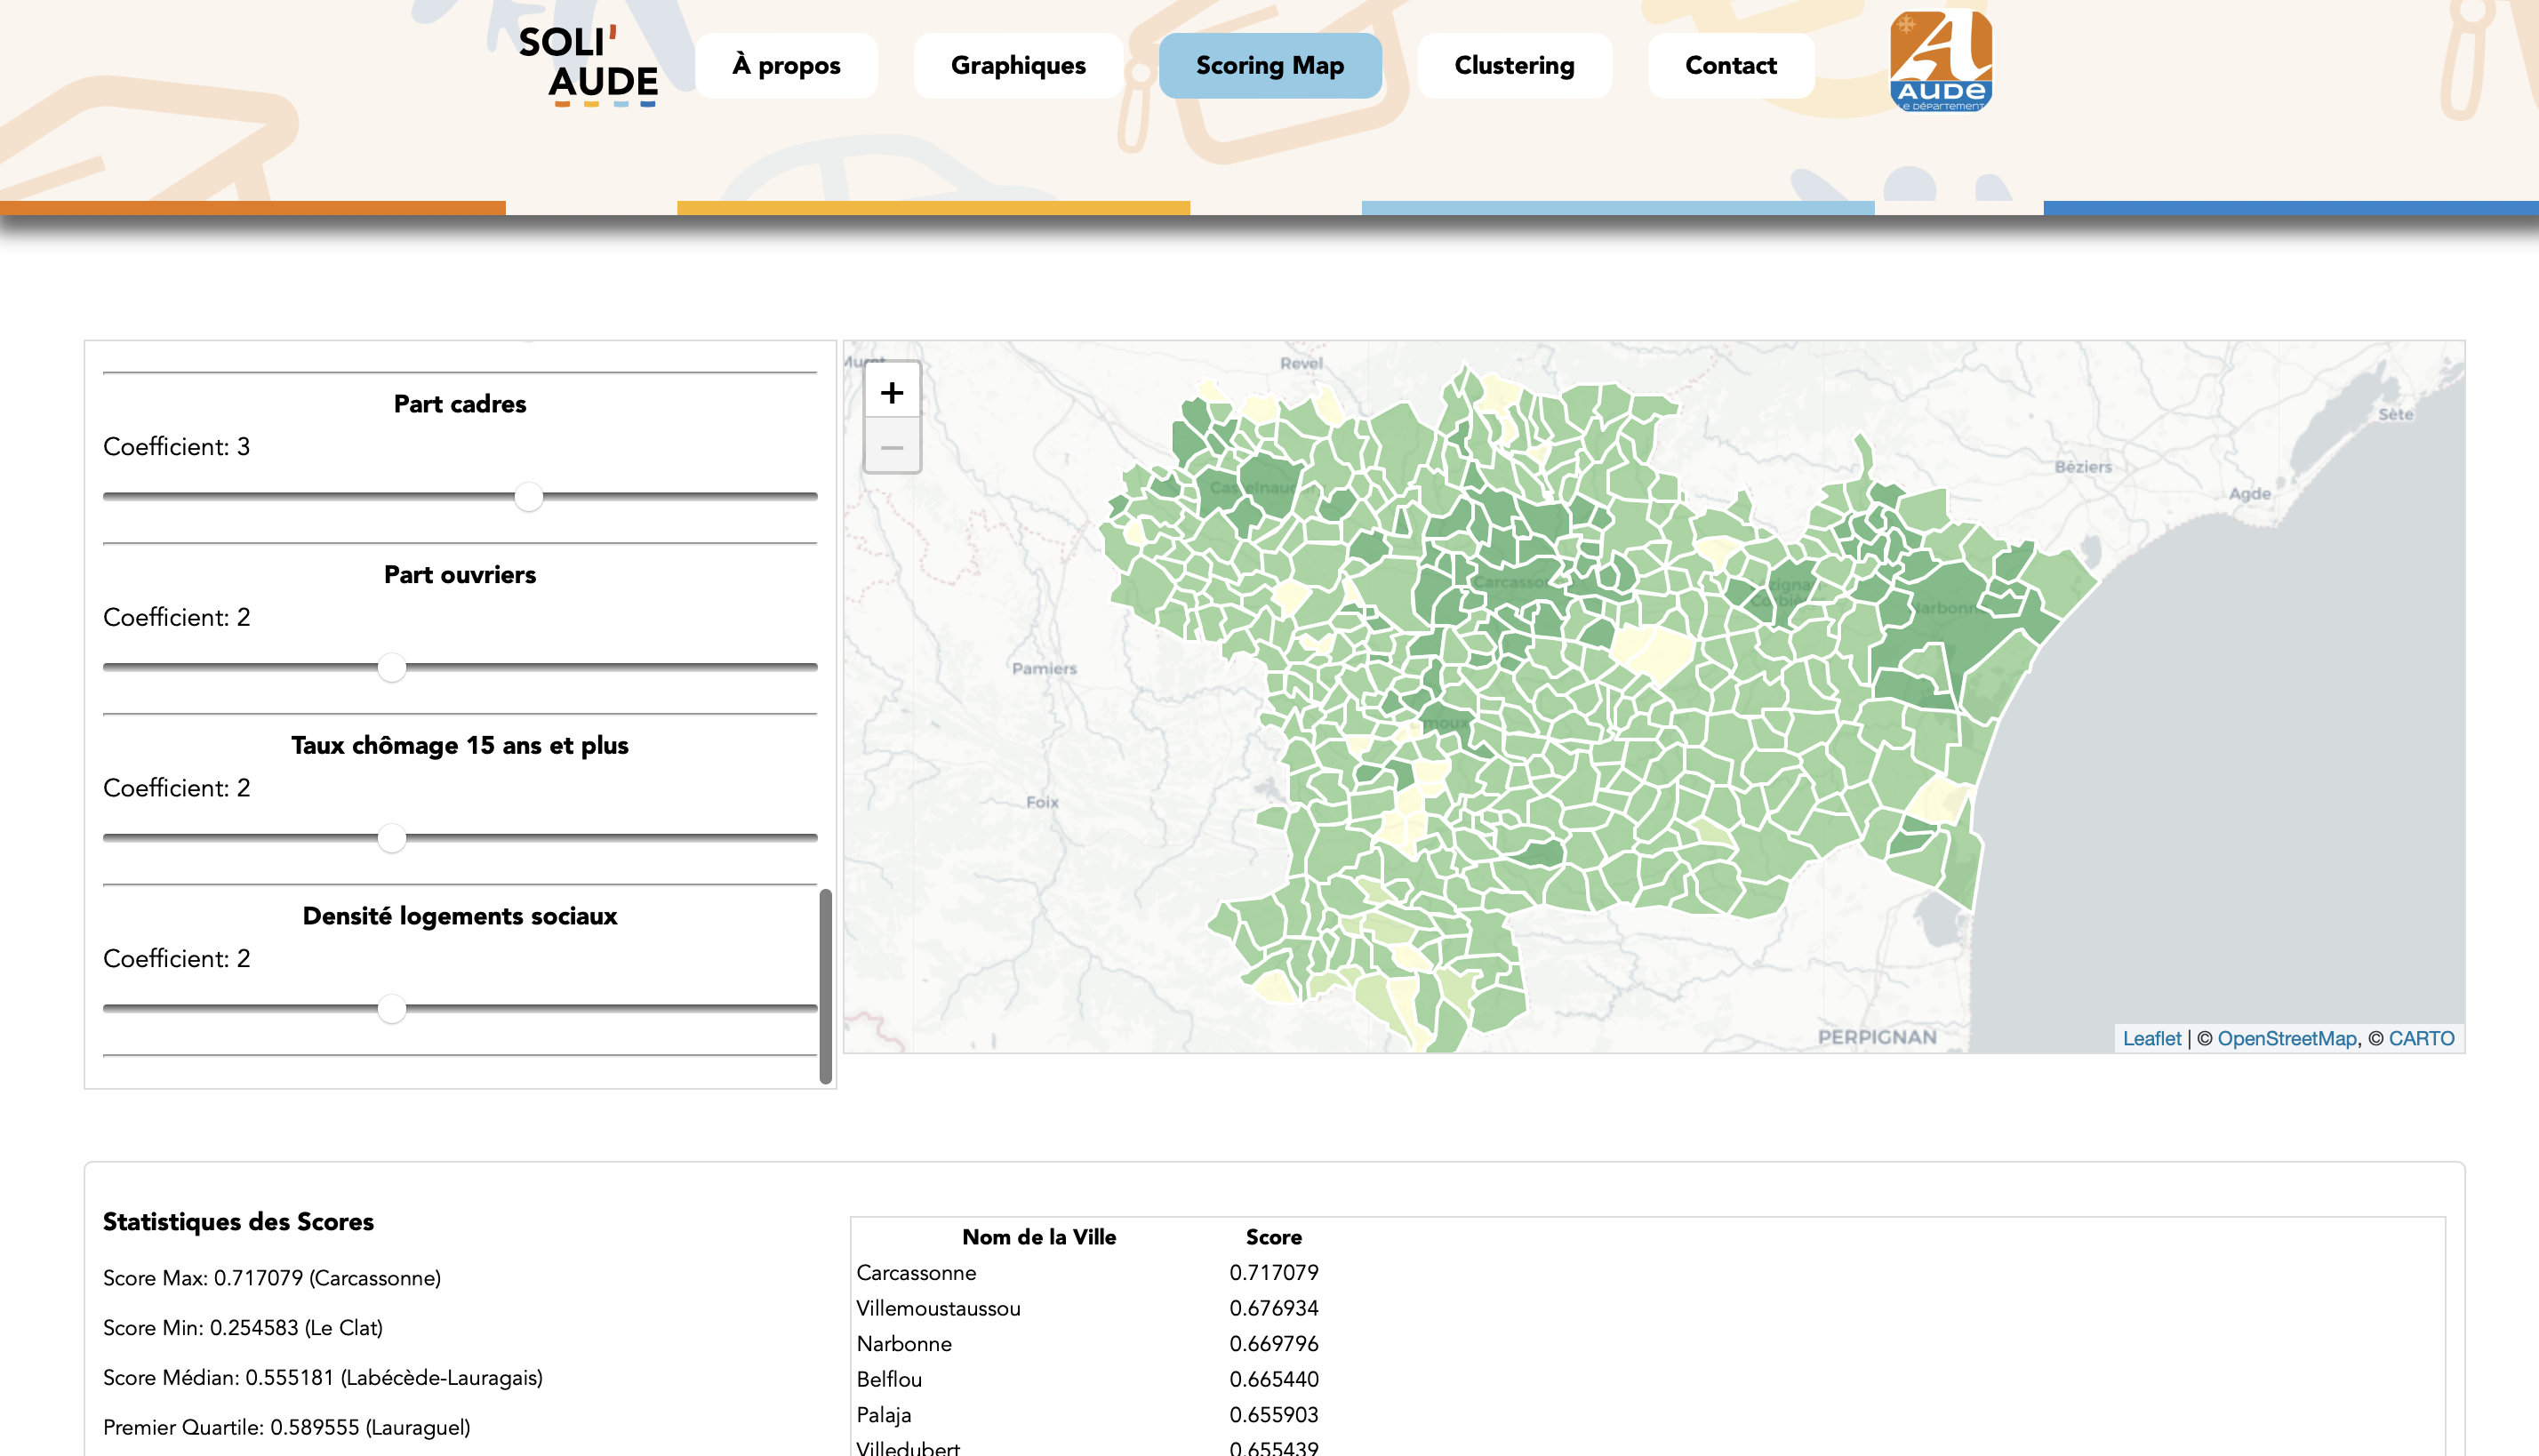
\includegraphics[width=0.6\textwidth]{2.png}
    \caption{Onglet indicateur}
    \label{fig:Site}
\end{figure}

Nous avons créé l'onglet permettant d'utiliser l'indicateur intéractif. Les coefficients impactent l'indicateur. Il est possible de consulter le classement qui s'adapte en fonction des valeurs des scores. 

\begin{figure}[h]
    \centering
    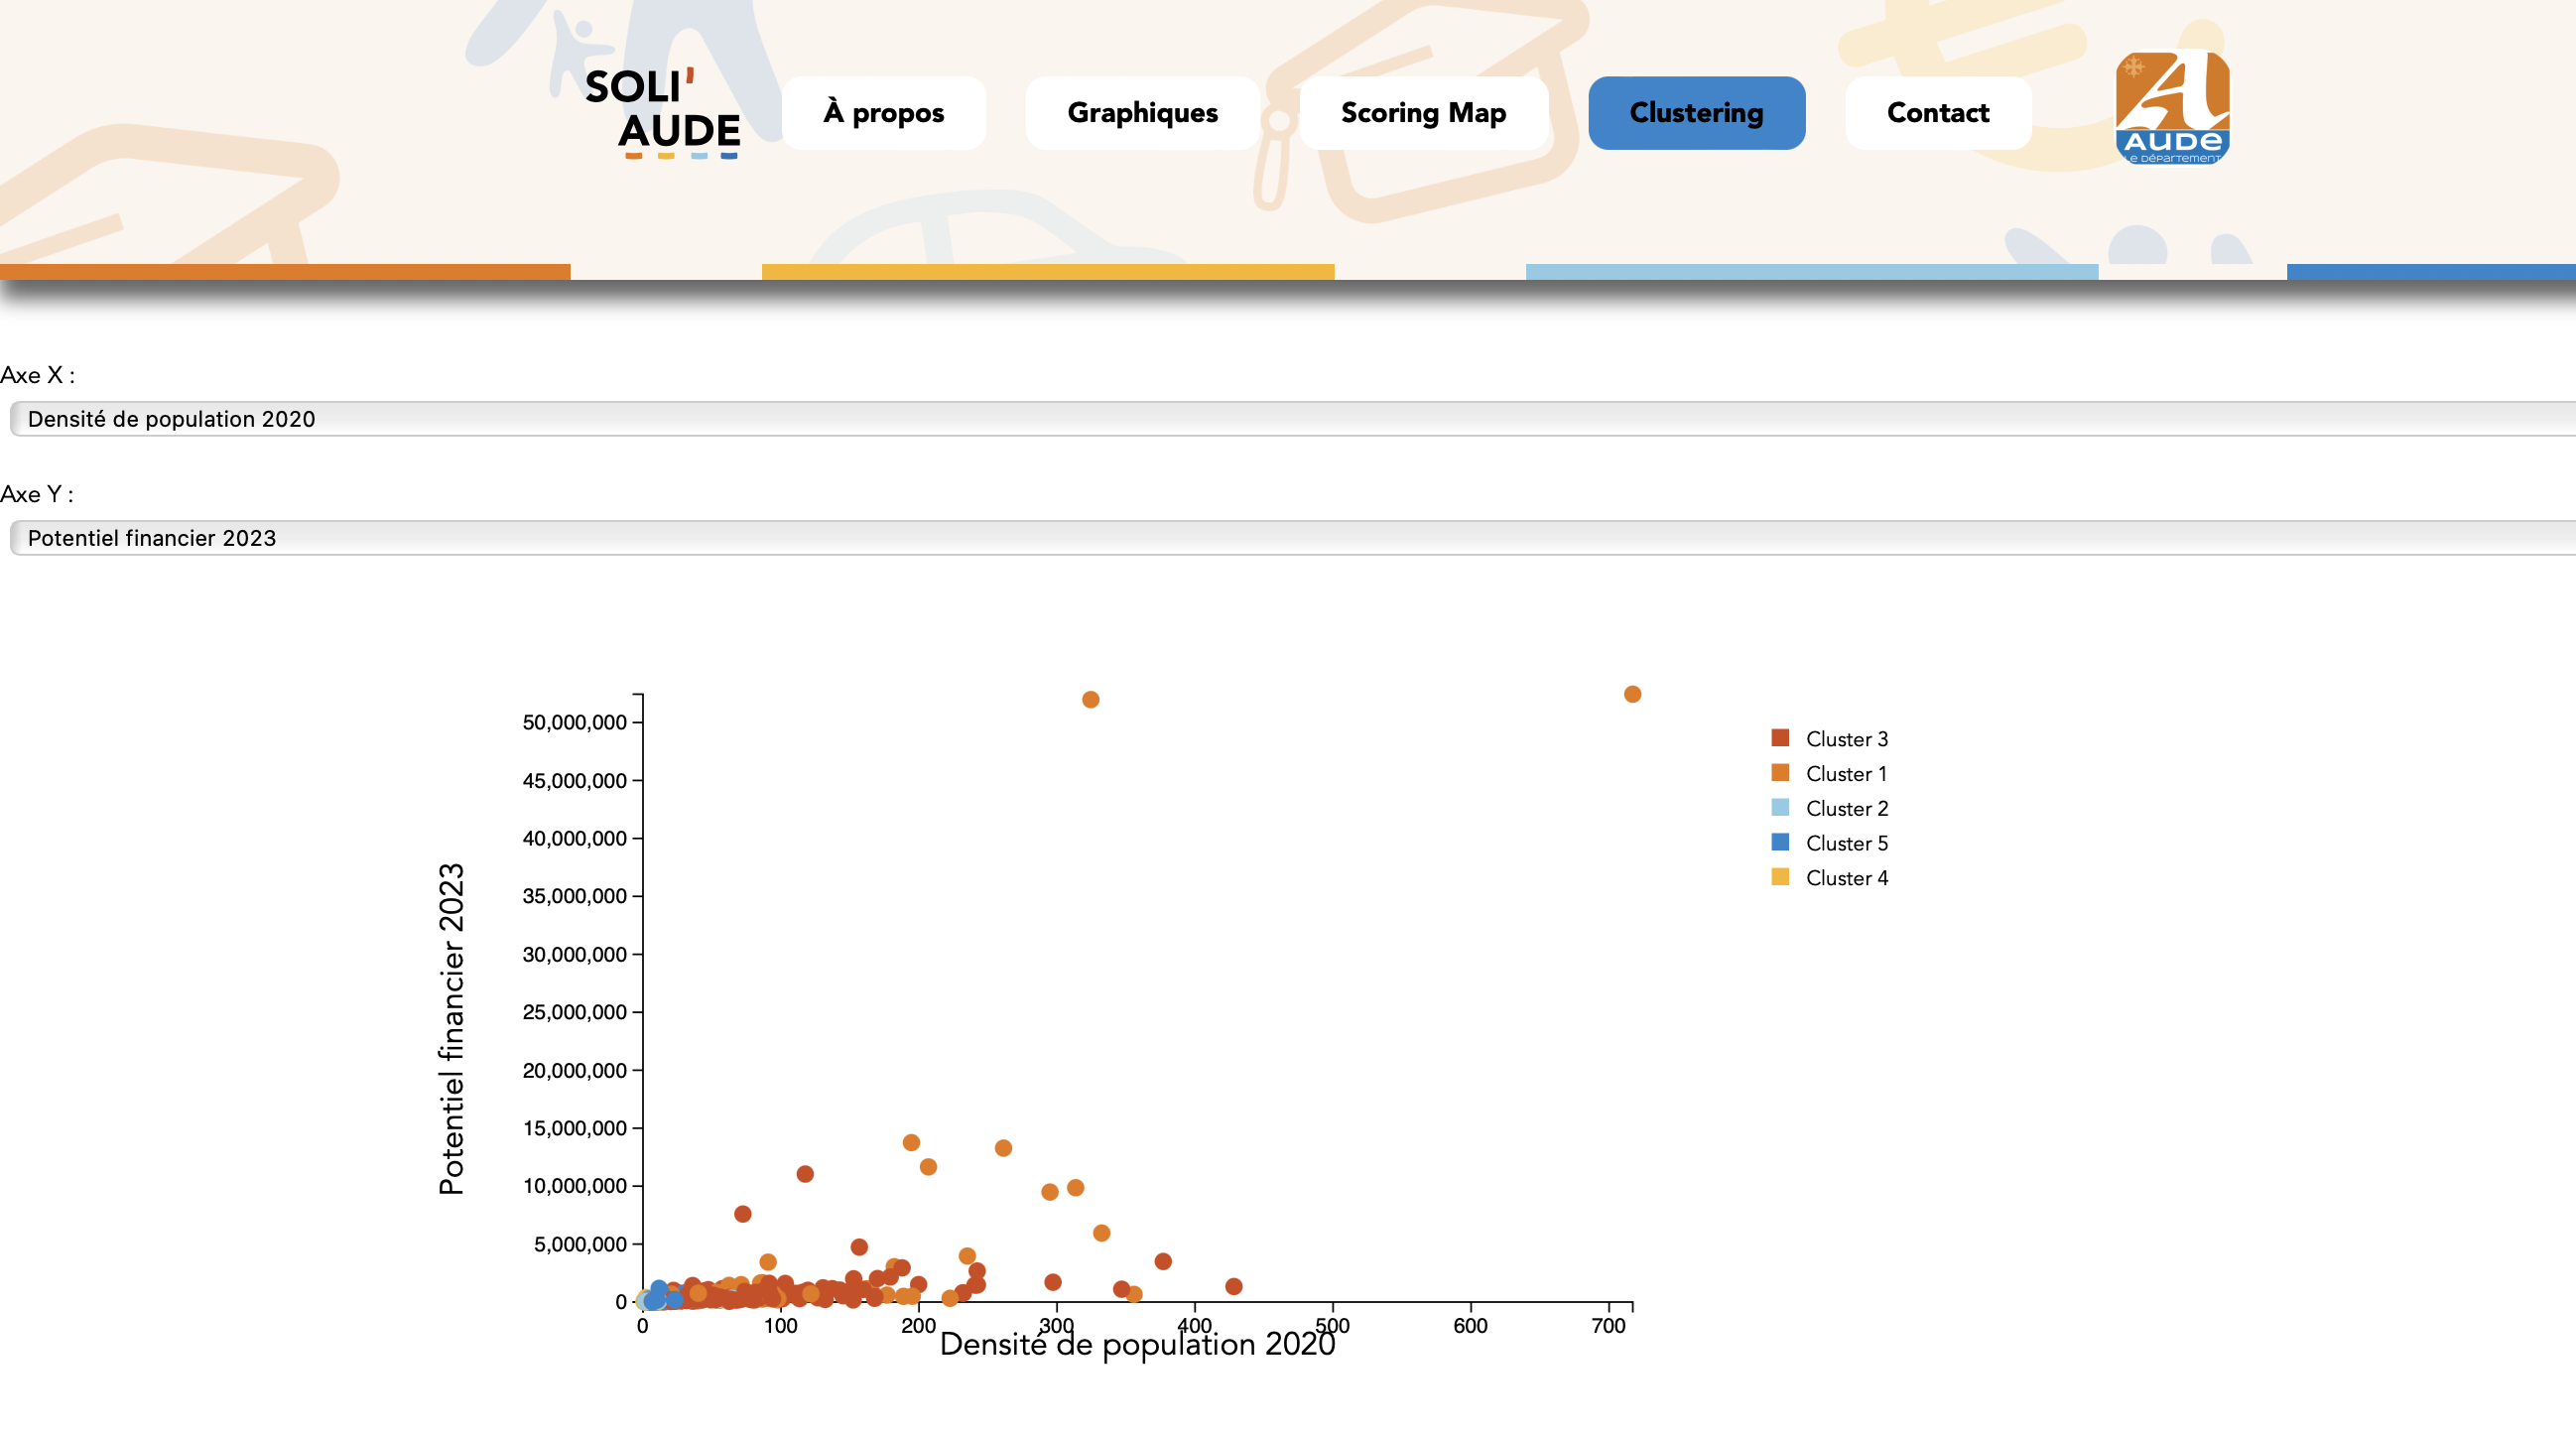
\includegraphics[width=0.6\textwidth]{3.png}
    \caption{Clustering}
    \label{fig:Clustering}
\end{figure}
\vspace{20cm}

Nous avons rajouté l'onglet clustering qui est actuellement en cours de développement mais nous ne savons pas si nous aurons le temps de la finir. Celle permet de visualiser la distribution des variables pour les 5 groupes de communes. 

\begin{figure}[h]
    \centering
    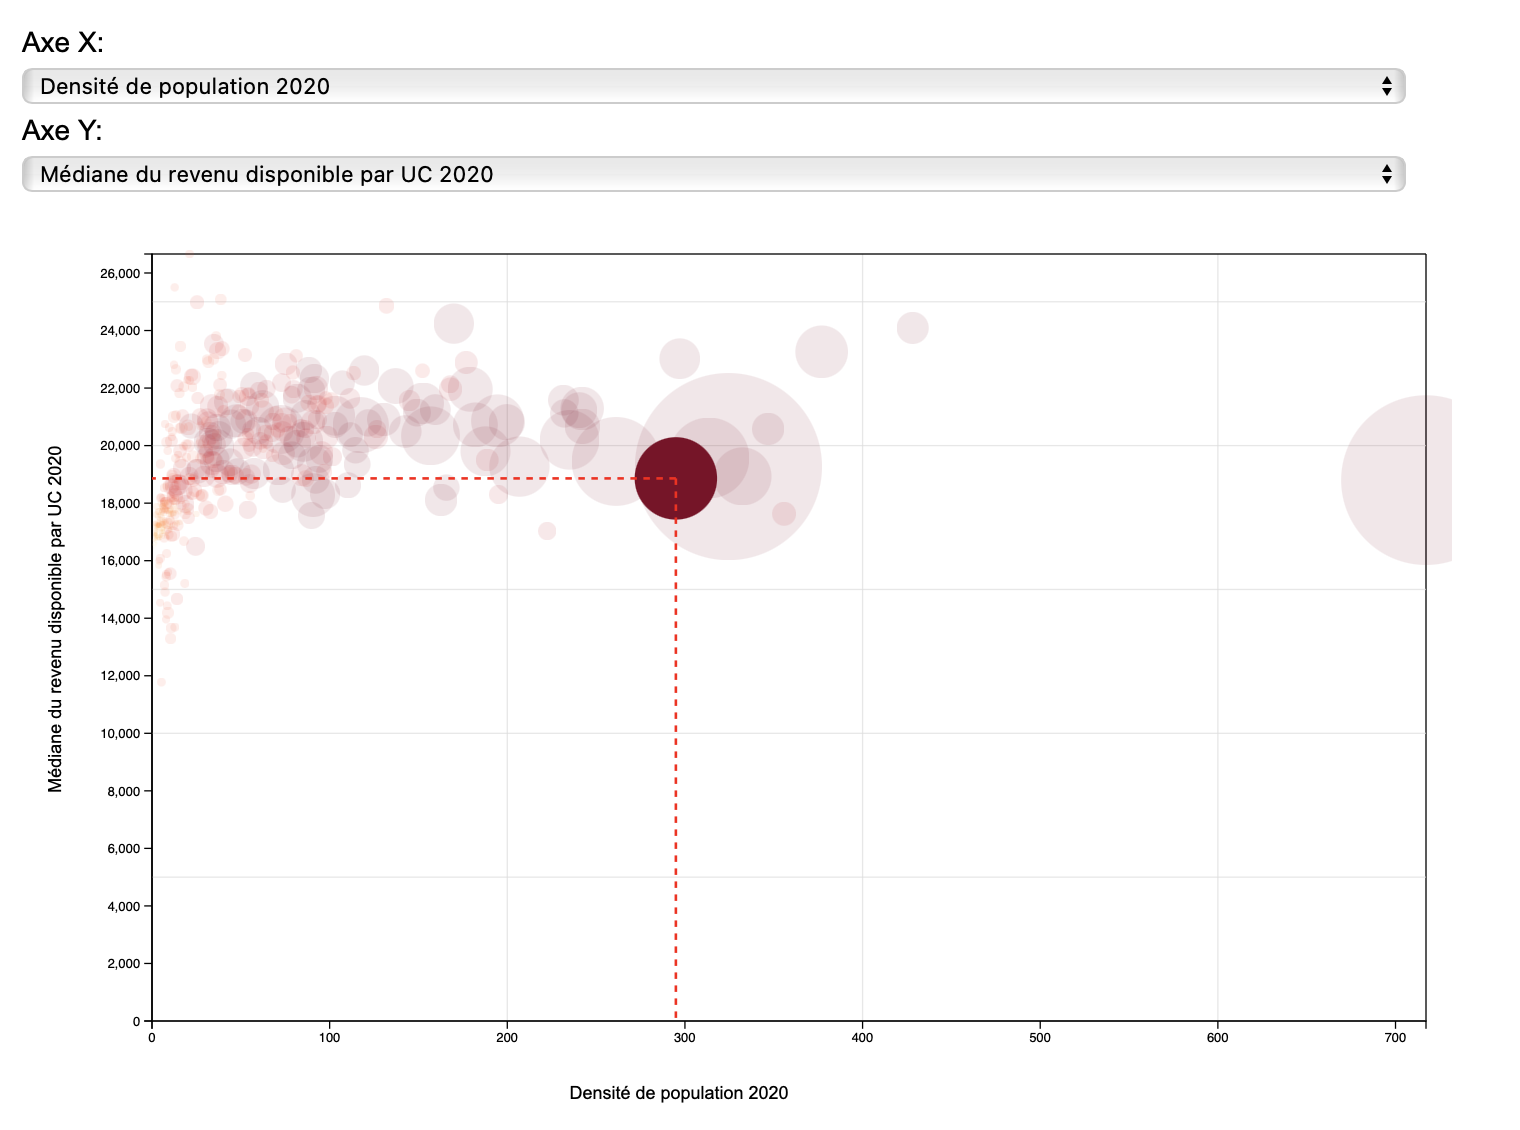
\includegraphics[width=0.6\textwidth]{4.png}
    \caption{Graphique en bulles}
    \label{fig:Graphique en bulles}
\end{figure}

\begin{figure}[h]
    \centering
    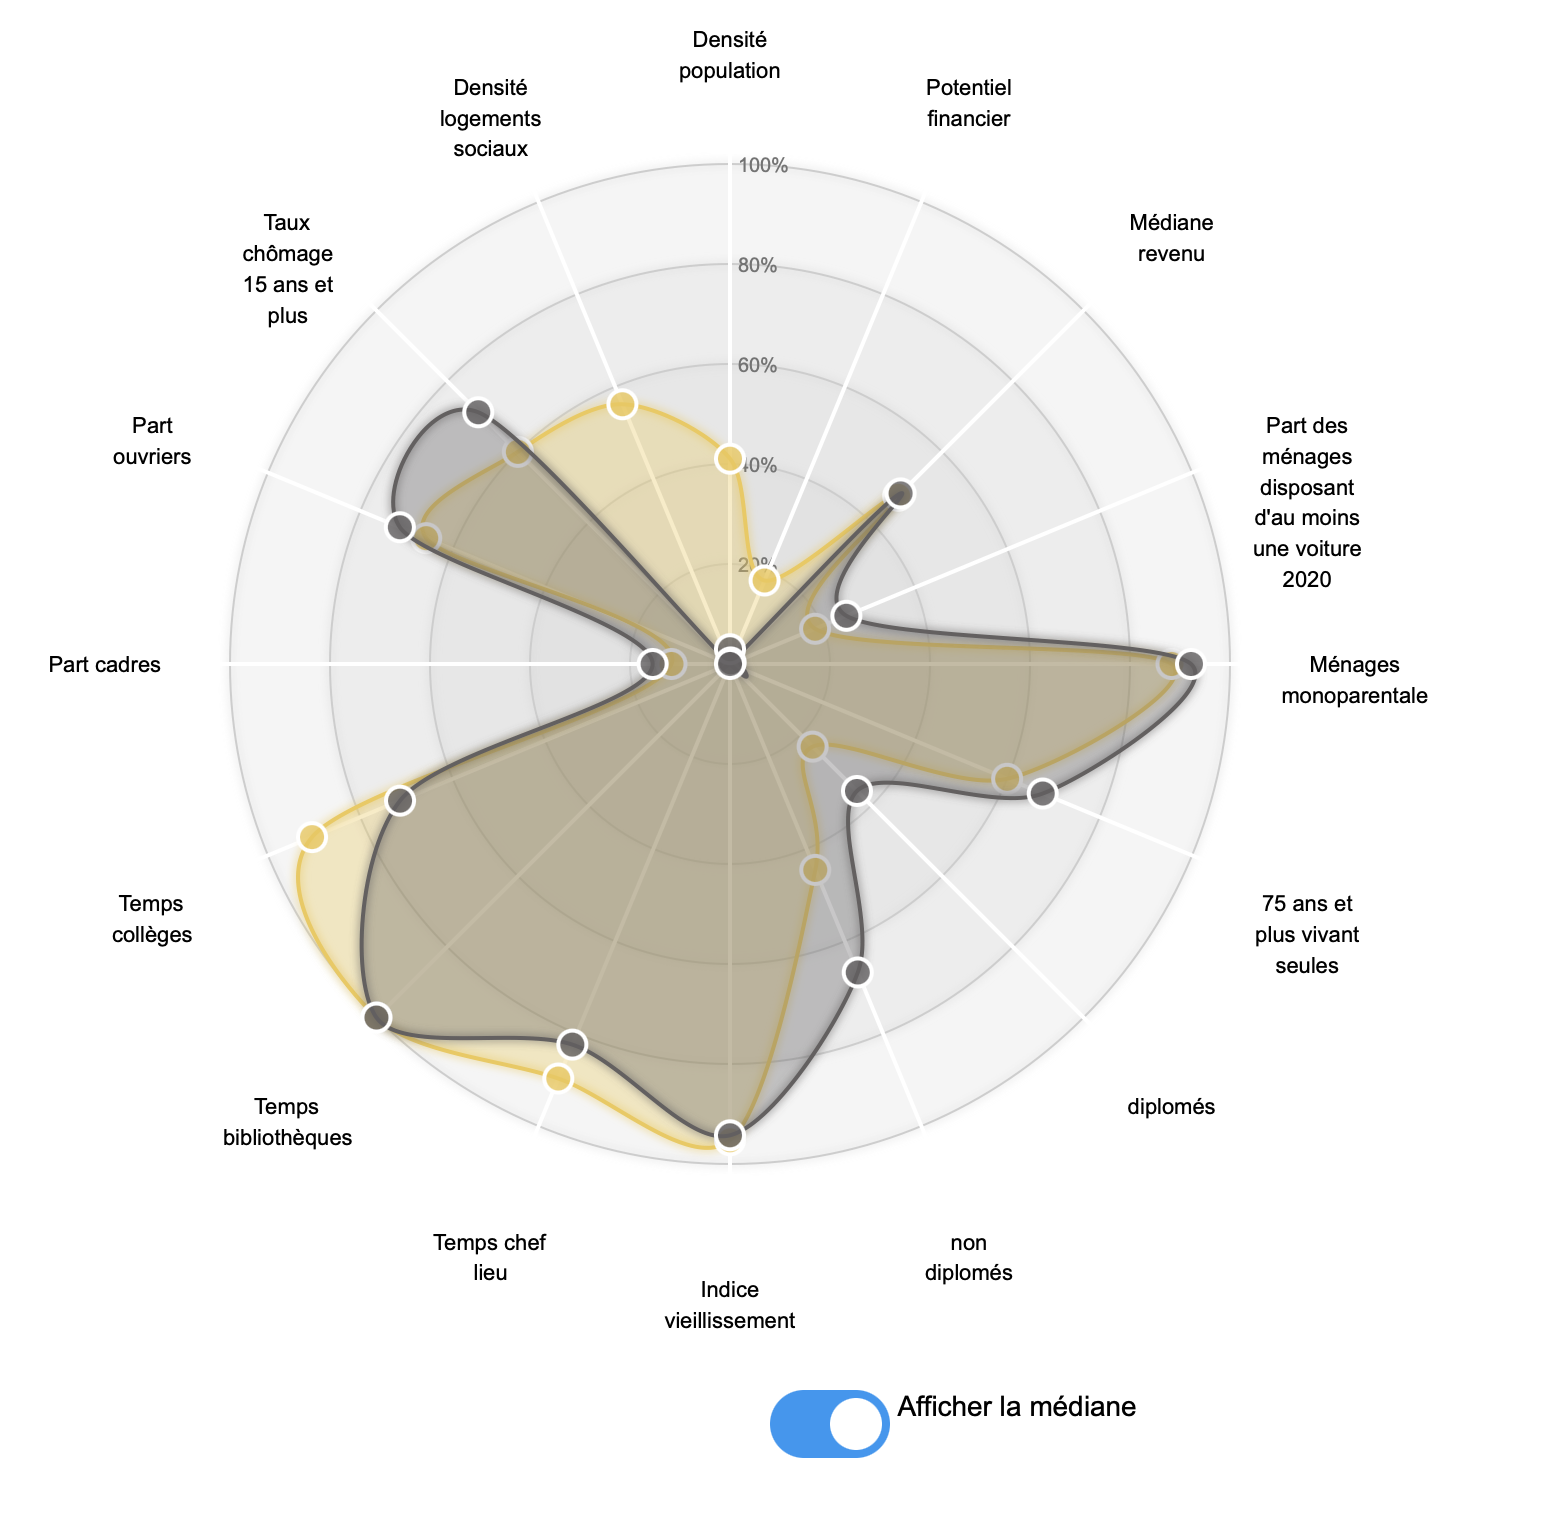
\includegraphics[width=0.6\textwidth]{6.png}
    \caption{Radar plot}
    \label{fig:Radar plot}
\end{figure}

\vspace{20cm}

Nous avons réussis à intégrer les liens entre les visualisations. Le radar a posé de nombreux problèmes techniques mais finalement, nous sommes plutôt satisfait du rendu. 


\section{Travail à faire}
\begin{itemize}
    \item Rajouter des descriptions pour chaque onglet permettant de mieux comprendre et utiliser les outils de visualisation.
    \item Vidéo de démo du site.
\end{itemize} 


\end{document}


